\documentclass[tikz,border=10pt]{standalone}
\usepackage{tikz}
\usetikzlibrary{positioning}

\begin{document}

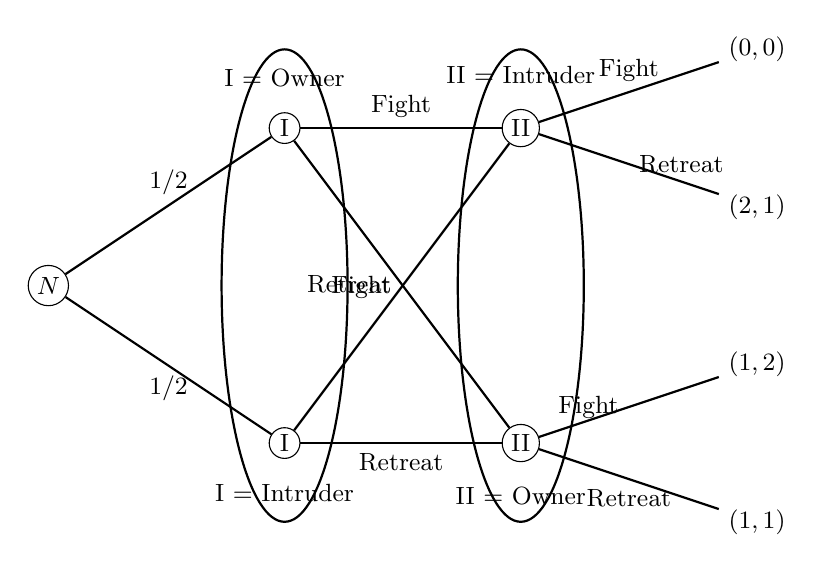
\begin{tikzpicture}[
    font=\small,
    decision/.style={circle,draw,inner sep=1.5pt},
    chance/.style={circle,draw,inner sep=1.5pt},
    terminal/.style={circle,fill,inner sep=1.2pt},
    line/.style={thick}
]

% Nature
\node[chance] (N) at (0,0) {$N$};

% Role assignment
\node[decision] (Aown) at (3,2) {I};
\node[decision] (Aout) at (3,-2) {I};

\node[decision] (Bown) at (6,2) {II};
\node[decision] (Bout) at (6,-2) {II};

% Nature moves
\draw[line] (N) -- node[above] {$1/2$} (Aown);
\draw[line] (N) -- node[below] {$1/2$} (Aout);

\node[above=2mm of Aown] {I = Owner};
\node[below=2mm of Aout] {I = Intruder};

\node[above=2mm of Bown] {II = Intruder};
\node[below=2mm of Bout] {II = Owner};

% Player I actions
\draw[line] (Aown) -- node[above] {Fight} (Bown);
\draw[line] (Aown) -- node[left] {Retreat} (Bout);

\draw[line] (Aout) -- node[left] {Fight} (Bown);
\draw[line] (Aout) -- node[below] {Retreat} (Bout);

% Player II actions
\node (T1) at (9,3) {$(0,0)$};
\node (T2) at (9,1) {$(2,1)$};
\node (T3) at (9,-1) {$(1,2)$};
\node (T4) at (9,-3) {$(1,1)$};

\draw[line] (Bown) -- node[above] {Fight} (T1);
\draw[line] (Bown) -- node[right] {Retreat} (T2);

\draw[line] (Bout) -- node[left] {Fight} (T3);
\draw[line] (Bout) -- node[below] {Retreat} (T4);

% Information sets
\draw[line] (3,0) ellipse (0.8 and 3);
\draw[line] (6,0) ellipse (0.8 and 3);

\end{tikzpicture}

\end{document}
